% --------------------------------------------------------------
% This is all preamble stuff that you don't have to worry about.
% Head down to where it says "Start here"
% --------------------------------------------------------------
 
\documentclass[12pt]{article}
 
\usepackage[margin=1in]{geometry} 
\usepackage{amsmath,amsthm,amssymb}
 
\newcommand{\N}{\mathbb{N}}
\newcommand{\Z}{\mathbb{Z}}
 
\newenvironment{theorem}[2][Theorem]{\begin{trivlist}
\item[\hskip \labelsep {\bfseries #1}\hskip \labelsep {\bfseries #2.}]}{\end{trivlist}}

\newenvironment{lemma}[2][Lemma]{\begin{trivlist}
\item[\hskip \labelsep {\bfseries #1}\hskip \labelsep {\bfseries #2.}]}{\end{trivlist}}

\newenvironment{exercise}[2][Exercise]{\begin{trivlist}
\item[\hskip \labelsep {\bfseries #1}\hskip \labelsep {\bfseries #2.}]}{\end{trivlist}}

\newenvironment{problem}[2][Part]{\begin{trivlist}
\item[\hskip \labelsep {\bfseries #1}\hskip \labelsep {\bfseries #2}]}{\end{trivlist}}

\newenvironment{intro}[2][Introduction]{\begin{trivlist}
\item[\hskip \labelsep {\bfseries #1}\hskip \labelsep {\bfseries #2}]}{\end{trivlist}}

\newenvironment{question}[2][Question]{\begin{trivlist}
\item[\hskip \labelsep {\bfseries #1}\hskip \labelsep {\bfseries #2.}]}{\end{trivlist}}

\newenvironment{corollary}[2][Corollary]{\begin{trivlist}
\item[\hskip \labelsep {\bfseries #1}\hskip \labelsep {\bfseries #2.}]}{\end{trivlist}}

\usepackage{graphicx}
\graphicspath{{./}}

\begin{document}
 
% --------------------------------------------------------------
%                         Start here
% --------------------------------------------------------------
 
\title{Project 1}%replace X with the appropriate number
\author{Yunzhong He\\ %replace with your name
204010749} %if necessary, replace with your course title
 
\maketitle

\begin{intro}{}
\item{}
In this project, we applied two dimension reductino techniques, PCA and FLD, on 178 faces with 256 x 256 pixels representing their appearances, and 87 x 2 points representing their landmarks. For part 1, we computed the eigenfaces on appearance and geometry, and examined reconstruction errors under diferent eigenspaces. We also randomly sampled some faces using the eigenfaces, using Gaussian distributions with their corresponding variances. For part 2, we projected these faces onto their fisherface and used it to classify male and female faces.
\end{intro}

\begin{problem}{1. ASM and AAM model for face reconstruction}
\item {1.}
For a total of 177 faces, we used 150 faces as the training set and computed their principle components as follows.\\\\
Let $\textbf{X}$ be a $150$ x $256^2$ matrix storing all the training images, we first computed the average face $\mu_X$. The result is below.
\begin{center}
		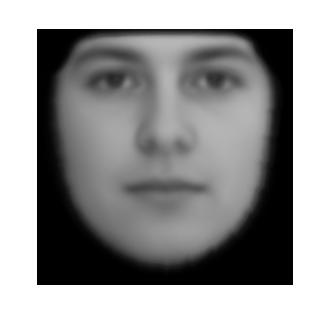
\includegraphics[height=5cm]{avgface.jpg}{\\fig.1 average face}
\end{center}
Then let $\textbf{S} = \textbf{X} - \mu_X$ and we performed eigenvalue decomposition of $\textbf{X}$'s covariance matrix $cov(\textbf{X})=\textbf{S'S}=\textbf{UDU'}$, and thus $\textbf{U}$ is the matrix storing all the principle components. Let all of the eigenvectors be sorted in decreasing order with regard to their eigenvalues, it can be shown that \textbf{U} minimizes reconstruction error $|\textbf{U}_k \textbf{U}_k'(v-\mu_x)+\mu_x - v|$ for image $v$.\\
But since $\textbf{S'S}$ is too large to be stored in Matlab, we instead computed eigenvalue decomposition of $\textbf{SS'}$ and multiplied its eigen-basis by $\textbf{S'}$ to obtain $\textbf{U}$. Below are the first 20 eigenfaces.\\
\begin{center}
		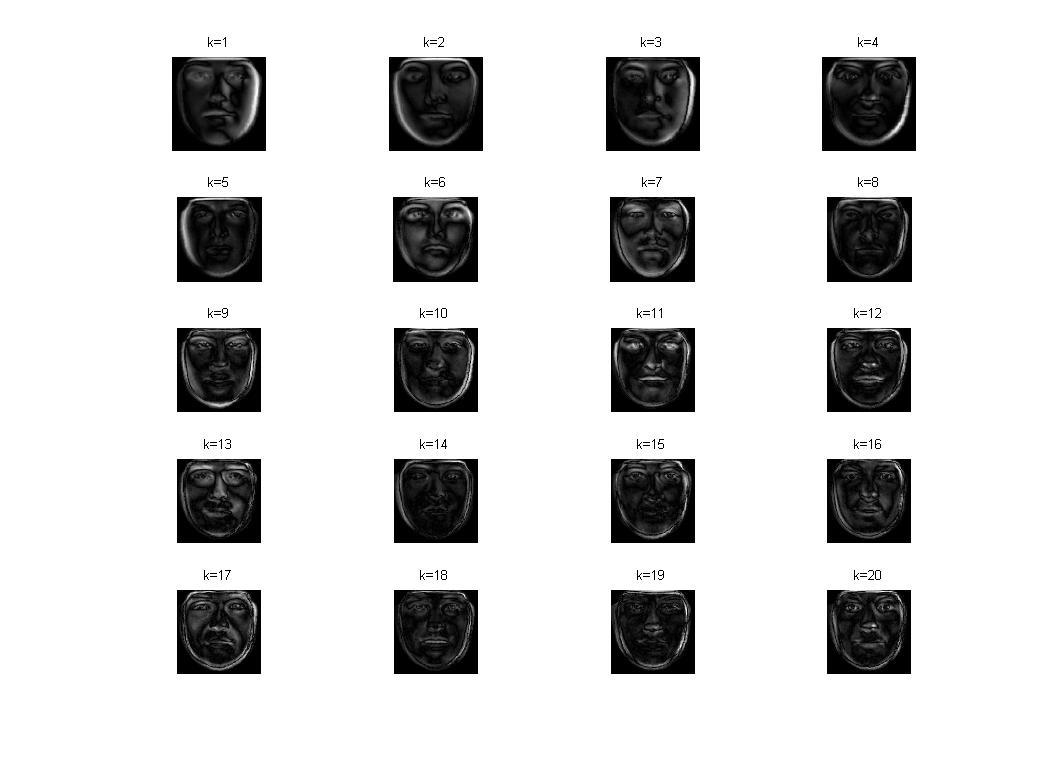
\includegraphics[height=10cm]{eigenfaces.jpg}{\\fig.2 eigenfaces}
\end{center}
From the eigenfaces above we can see that some areas are hightlighted, meaning they are parts of faces that best characterizes a human face. And they seem to have a correspondence with muscles of a face.
\\\\We then reconstructed the faces using their first k eigenvectors, and calcuated the average sum of squared error per pixel. Below is the reconstruction error with regard to different values of k.\\
\begin{center}
		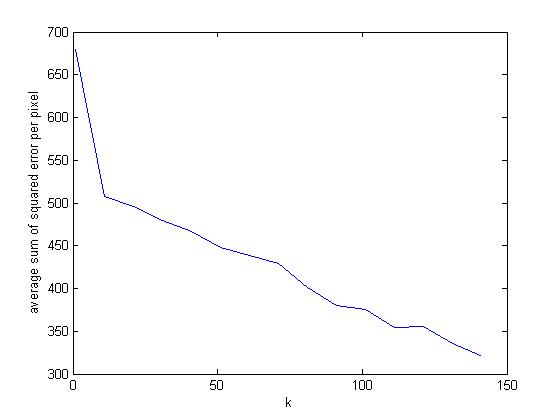
\includegraphics[height=8cm]{error_face.jpg}{\\fig.3 reconstruction errors}
\end{center}
We can see that the error curve drops significantly when adding the first few eigenvectors, this makes sense because they have the largest corresponding eigenvalues, and thus constribute the most to the reconstructions.\\
\item{2.}
Similarly, using the same approach for landmarks we obtain the average landmark, and the error curve as follows.\\
\begin{center}
		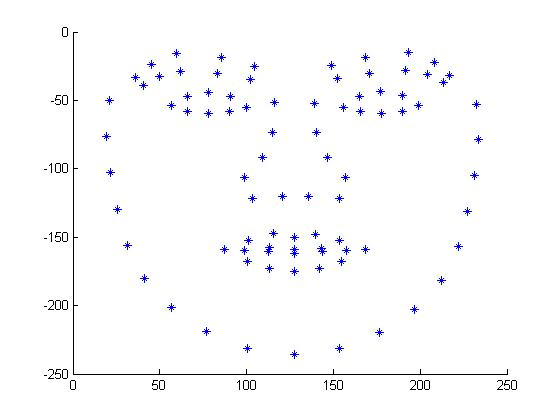
\includegraphics[height=8cm]{avglandmark.jpg}{\\fig.4 eigenlandmarks}
\end{center}
\begin{center}
		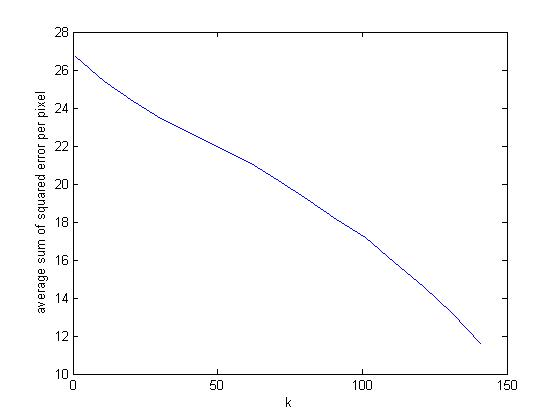
\includegraphics[height=8cm]{error_landmark.jpg}{\\fig.5 reconstruction errors}
\end{center}
The error drops more smoothly in this case, which suggests that the eigenvalues of landmarks's principle components are close. This confirms with the eigenvalues that we found.\\
\item{3.}
Combining the steps above, for each test image, we first encoded their aligned appearance by projecting onto the principle components from (1), then encoded their landmarks by projecting their landmarks onto principle components from (2). We then reconstructed apppearance appearance like in (1), and reconstructed the landmarks like in (2), and aligned the reconstructed appearance back to its recostructed landmarks. Under different values of k, we have the following reconstruct errors.
\begin{center}
		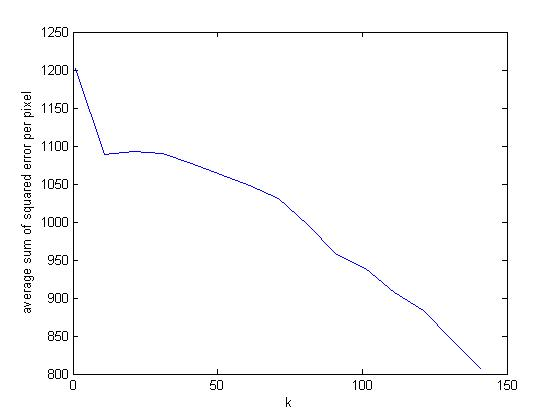
\includegraphics[height=8cm]{error_warp.jpg}{\\fig.6 reconstruction errors}
\end{center}
Notice that the errors are slightly larger than we had without warping, and it may due to the additional reconstruction error that come from landmarks.
\item{4.}
		Assuming both appearances and landmarks follow Gaussian distributions around their principle components, we randomly sampled some images with different variance. For the first 20 faces below, we sampled appearance and geometry with their corresponding variances. For the second 20 faces below, we changed $\sigma_{landmark}^2$ to larger values and obtained some funny faces.
\begin{center}
		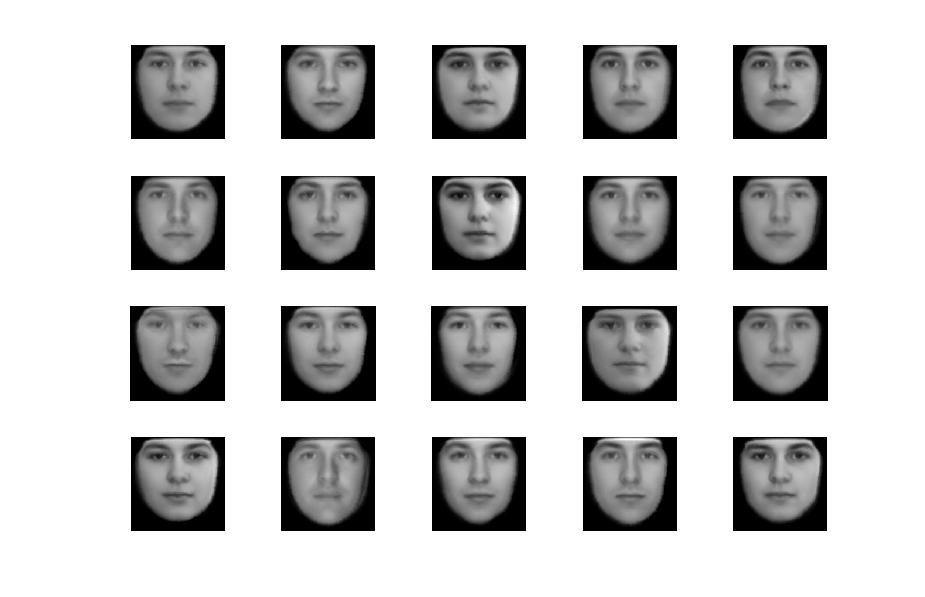
\includegraphics[height=8cm, width=12cm]{rand_face_true.jpg}{\\fig.7 random faces sampled with corresponding eigenvalues}
\end{center}
\begin{center}
		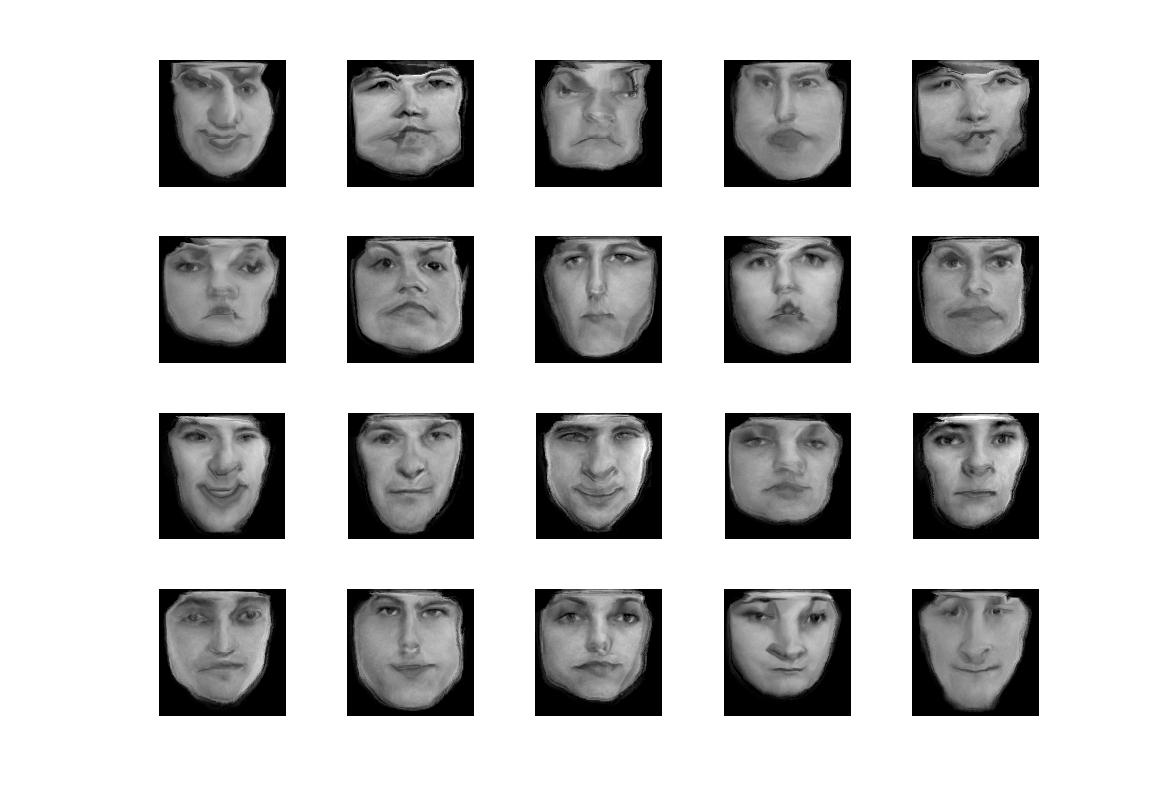
\includegraphics[height=8cm, width=12cm]{rand_face_funny.jpg}{\\fig.8 random faces sampled with larger variances}
\end{center}
\end{problem}

\begin{problem}{2. Fisher faces for gender discrimination}
\item{5.}
For the 88 male and 85 female faces dataset, we first aligned them to the average landmark, then applied FLD on 78 male faces and 75 female faces to find the axis $\omega$ that best distinguishes male and females faces, such that
\begin{align*}
		\textbf{S}_B \omega_i = \lambda_i \textbf{S}_W \omega_i
\end{align*}
where $\textbf{S}_B$ is the between class scatter matrix, and $\textbf{S}_W$ is the within class scatter matrix. And we applied a similar trick like in Part 1 to work with large matrices in order to solve for $\omega$. Below is the projection of all the test data onto $\omega$
\begin{center}
	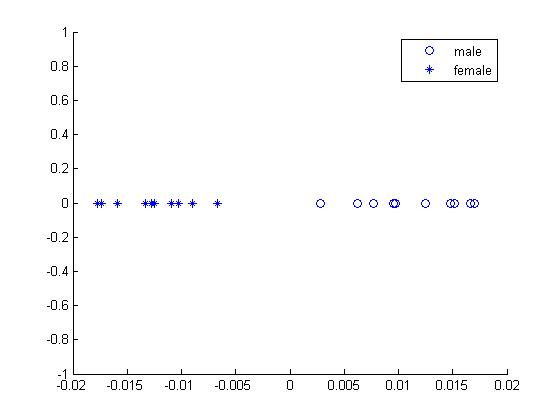
\includegraphics[height=8cm]{projection.jpg}{\\fig.9 test faces projection}
\end{center}
We can see that the two classes are separated very well, indicating that the classification should be pretty accurate. Apply KNN classification with regard to 4 nearest neighbors, we achieved \textbf{100\%} accuracy on the remaining 20 images. However, if we reduce the training set to 18 males and 15 females, the KNN accuracy drops to around \textbf{77\%}.\\

\item{6.}
Instead of finding $\omega$ for aligned images, we find fisher faces both for appearance and landmarks, with 78 male faces and 75 female faces as the traning set. Then we projected the appearance and landmark of the remaning 20 images to the axies, so that every face can be represented by two real numbers. And we obtained the following figure.
\begin{center}
	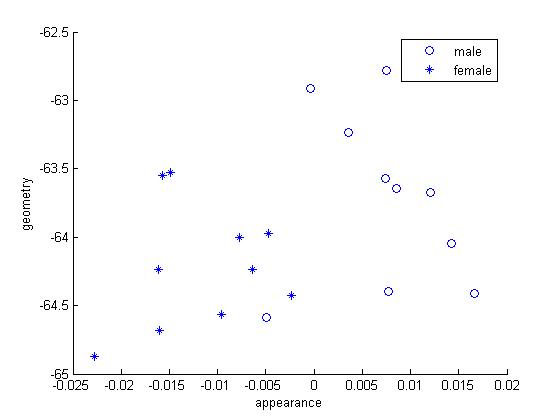
\includegraphics[height=8cm]{visualization.jpg}{\\fig.10 faces 2D projection}
\end{center}
We can see that the two classes are well-separated, except for one outliers from the male faces. This explains the accuracy of KNN algorithm in (5). And below is the outlier, which indeed looks like a female face in some sense.
\begin{center}
	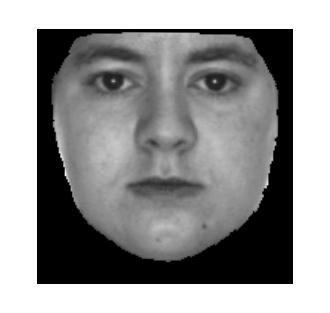
\includegraphics[height=5cm]{outlier.jpg}{\\fig.11 outlier}
\end{center}

\end{problem}

% --------------------------------------------------------------
%     You don't have to mess with anything below this line.
% --------------------------------------------------------------
 
\end{document}
